\chapter{Felhasználói dokumentáció}
\label{ch:user}

A következő fejezetben fogom bemutatni az alkalmazás elérését, egyes komponenseit, illetve felhasználási lehetőségeit. 

Ez a pénzügyeket rendszerező alkalmazás alapvetően magánszemélyeknek készült, személyes felhasználásra, de mivel lehetőséget nyújt csoportos használatra is, ezáltal akár egy kisebb vállalat igényeit is elláthatja.

A főbb funkciók közé tartozik, hogy bevételeket és kiadásokat lehet rögzíteni, kategóriák szerint csoportosítva, illetve kimutatásokat nézhet a felhasználó a pénzügyi szokásairól, melyeket exportálni is tudja. Az alkalmazás egyik nagy előnye, hogy nem csak egyének használhatják, hanem csoportok (például háztartások) is.


\section{Rendszerkövetelmények}

Mivel egy webes alkalmazásról van szó, ezért különleges gépigény nem szükséges. Szinte az összes böngésző támogatott.

\section{Felhasználói esetek}

Az alkalmazás felhasználói eseteit ez a bejegyzés fogja taglalni jobban, képernyőképekkel magyarázva.
\begin{table}[H]
	\centering
	\begin{tabular}{ | m{0.25\textwidth} | m{0.65\textwidth} | }
		\hline
		\textbf{Funkció} & \textbf{Leírás} \\
		\hline \hline
		\emph{Bejelentkezés} & Bejelentkezés egy egyedi felhasználónévvel és egy jelszóval lehetséges \\
		\hline
		\emph{Regisztráció} &  Quisque lobortis eros vitae urna lacinia euismod. \\
		\hline
		\emph{Elfelejtett jelszó} & Curabitur ac lacus pellentesque, eleifend sem ut, placerat enim. Ut auctor tempor odio ut dapibus. \\
		\hline
	\end{tabular}
	\caption{Maecenas tincidunt non justo quis accumsan}
	\label{tab:example-1}
\end{table}

\begin{figure}[H]
	\centering
	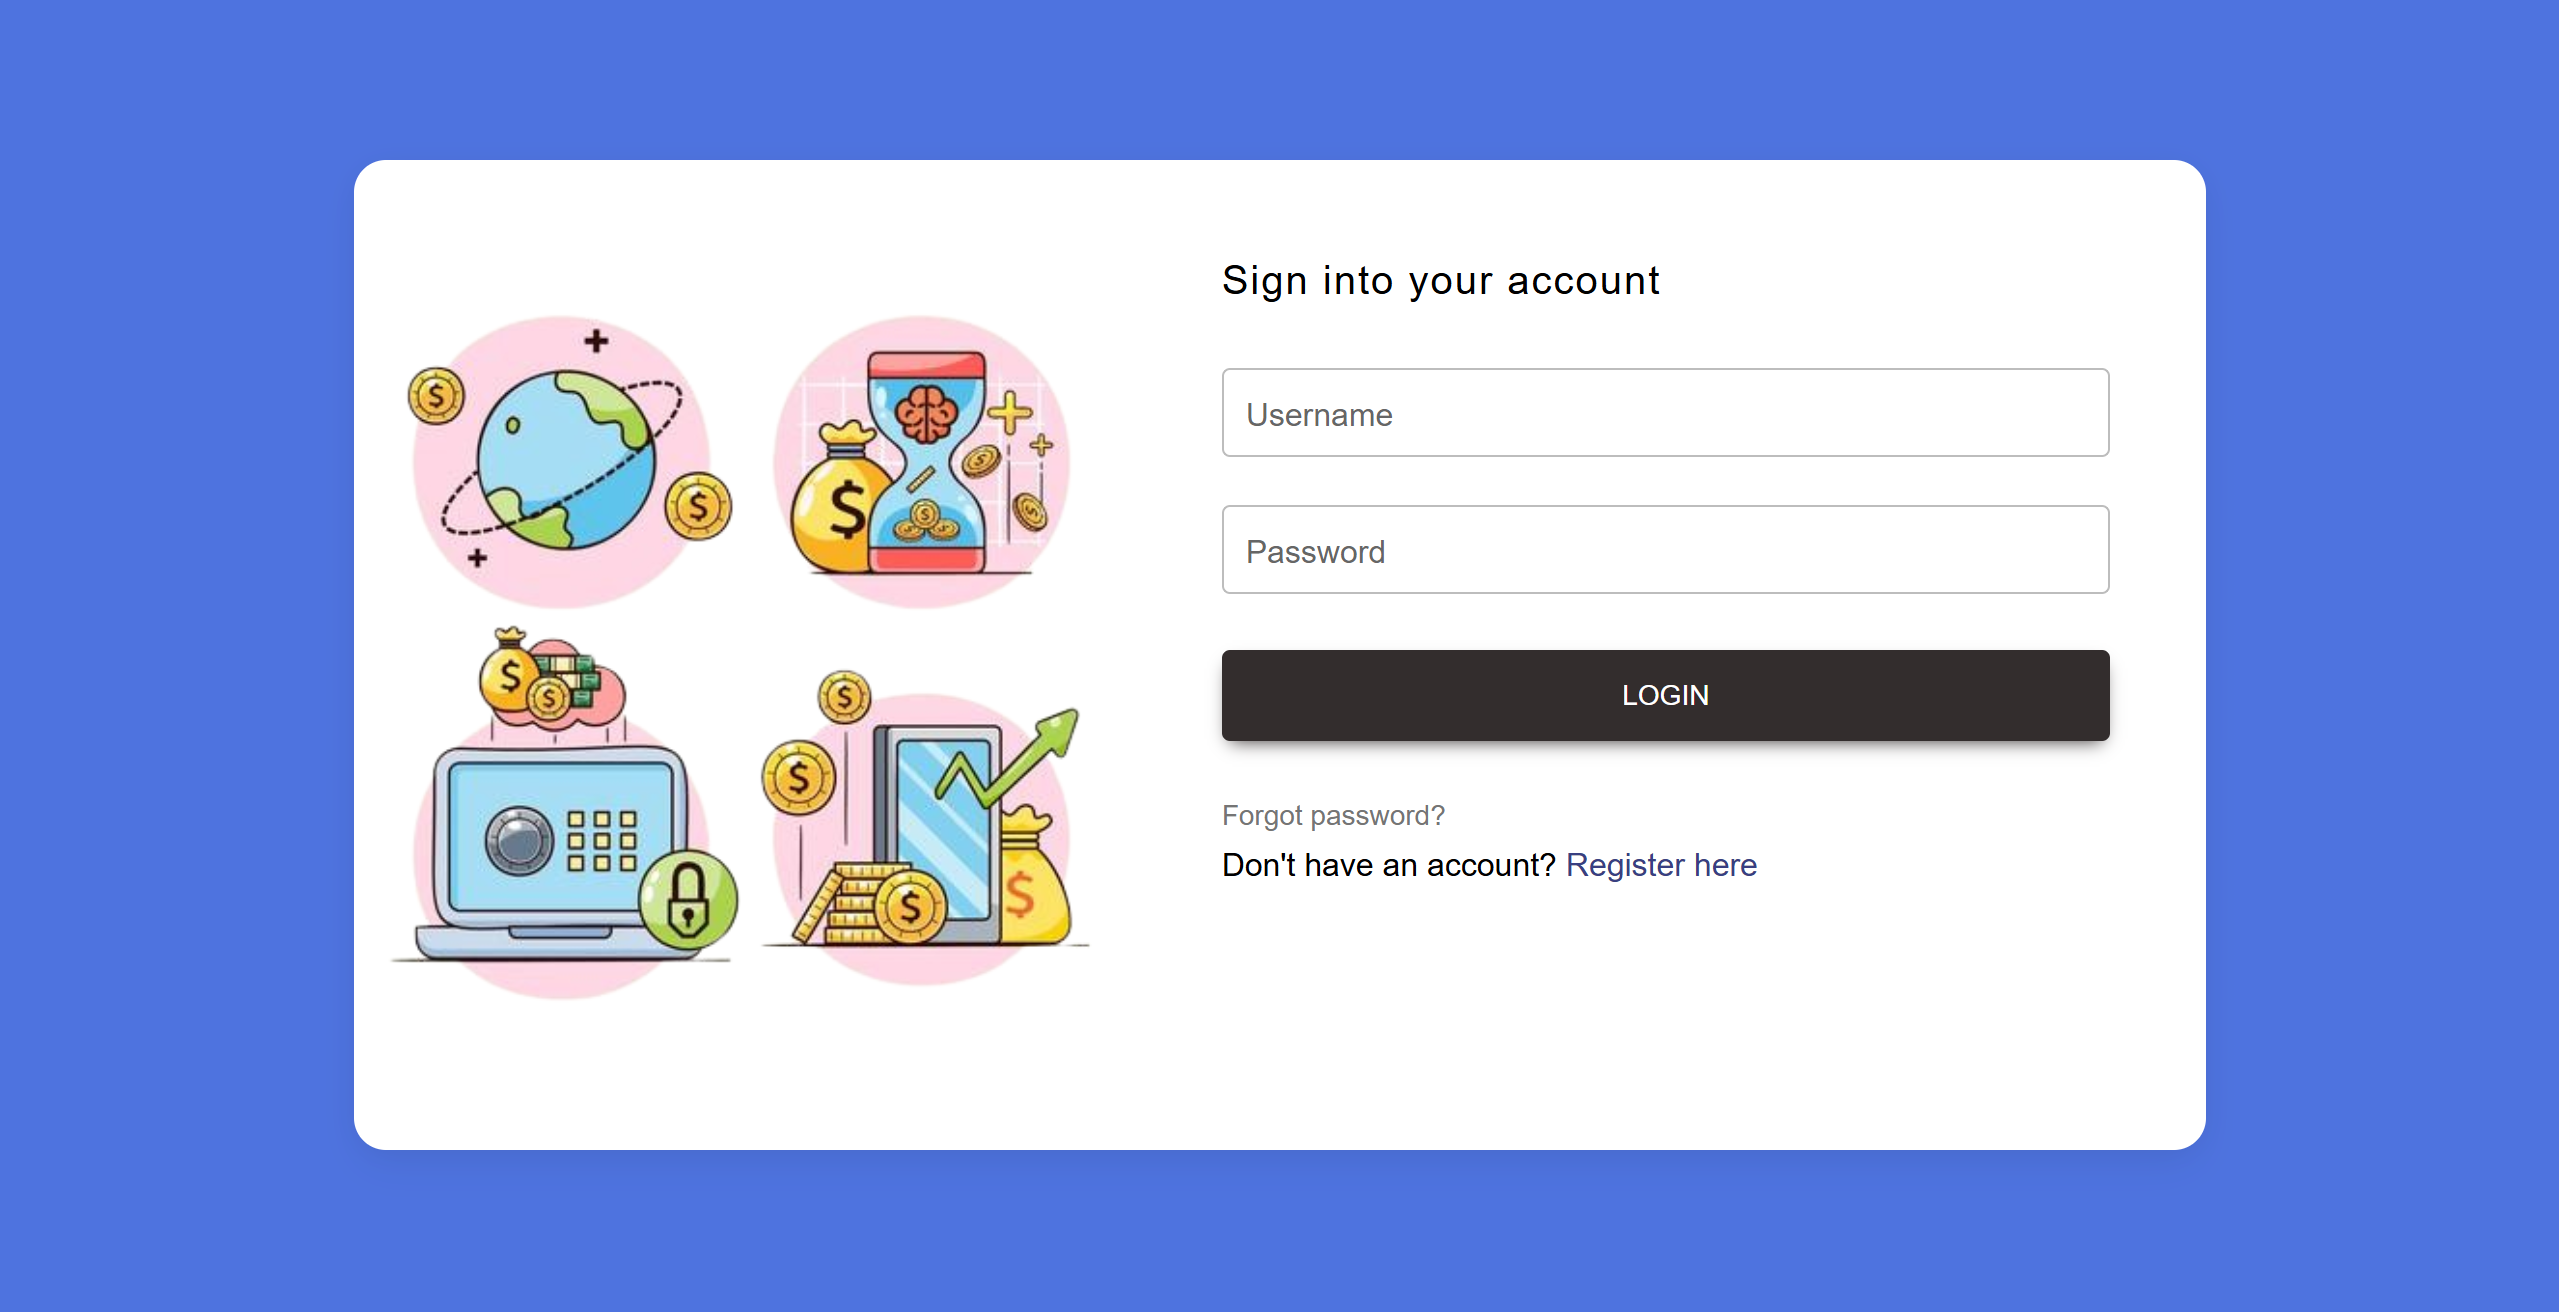
\includegraphics[height=180px]{img/login-screenshot}
	\caption{Screenshot: Bejelentkező felület}
	\label{fig:example-1}
\end{figure}
